% ====================================================================
%+
% SECTION:
%    MW_Astrometry.tex
%
% CHAPTER:
%    galaxy.tex
%
% ELEVATOR PITCH:
%
%-
% ====================================================================

\section{Astrometry with LSST: Positions, Proper Motions, and Parallax}
\def\secname{MW_Astrometry}\label{sec:\secname}

\credit{dgmonet}, \credit{DanaCD}, \credit{jgizis}, \credit{mliu},
\credit{caprastro}, \credit{willclarkson}, \credit{yoachim}

A number of Milky Way science cases of interest to the Astronomical
community will depend critically on the astrometric accuracy LSST will
deliver. While ``astrometry'' is not a science case in the framework
of this white paper, LSST's astrometric performance will be sensitive
to the particular choice of observing strategy.
%While astrometry is not a science case, high astrometric accuracy enables
%a large number of science cases.
Hence, the LSST Observing Strategy needs to be examined for systematic
trends that might limit or even preclude precise measures of
stellar positions, proper motions, parallaxes, and perturbations that
arise from unseen companions.

\autoref{sec:\secname:MW_Astrometry_measurements} highlights two
science cases at opposite scales of distance from the Sun that require
accurate and precise astrometry and/or proper motion
measurements. \autoref{sec:\secname:MW_Astrometry_metrics} presents
Metrics for LSST's astrometric performance, and discusses Figures of
Merit for the two highlighted science cases. These metrics are applied to two example OpSim runs in
\autoref{sec:\secname:MW_Astrometry_OpSim}. Finally in Section
\ref{sec:\secname:MW_Astrometry_furtherwork}, the work that is still
needed is discussed, both in terms of the Metrics and the Figures of
Merit that depend on them.

%Each of these cases stresses different aspects of the LSST hardware, software,and observing strategies.

%, here we highlight three representative science cases.
%that illustrate the various impacts of the observing strategy might
%be:
%To highlight the
%various astrometric impacts of the strategy, three science cases have
%been chosen for particular attention:

%\subsection{Introduction: Astrometry as a special case}
%\label{sec:\secname:MW_Astrometry_intro}

\subsection{Target Measurements and Discoveries}
\label{sec:\secname:MW_Astrometry_measurements}

%\begin{itemize}
%\item[1.] Identification of Streams in the Galactic Halo using proper motions.
%\item[2.] A complete sample of stars in the solar neighborhood.
%\end{itemize}
%\item The tie between the Radio and Optical realizations of the International Celestial Reference System.
%\item The specific and ensemble agreement between LSST and Gaia parallaxes.

{\bf 1. Identification of Streams in the Galactic Halo Using Proper Motions}

Much of the Milky Way's stellar halo was built by the accretion of smaller galaxies. Given that these galaxies
were generally of low mass, their tidal debris should still form coherent structures in phase space, especially
in the outer Galaxy where dynamical times are long. The identification of these streams would allow
a reconstruction of the accretion history of the Milky Way. Tides also lead to the dissolution of globular clusters,
leaving notably thin streams that serve as sensitive tracers both of the Galactic potential and of the presence of dark
subhalos.

A relatively small number of streams, originating from both dwarfs and globular clusters, have been identified via photometry
of individual stars in large surveys such as SDSS\@. However, only the highest surface brightness structures can be found
in this manner, and it is often difficult to trace the streams over their full extent. LSST will enable streams to be identified
by stellar proper motions, and combined with targeted follow-up spectroscopy, will yield full 6-D position and velocity measurements suitable for dynamical modeling.
Further, it will allow the discovery of tidal debris that is no longer spatially coherent but which can be unambiguously identified in phase space.

Finally, streams and other kinematically-distinct halo substructure
can be identified and characterized by combining proper motions and
photometry in reduced proper-motion diagrams \citep[e.g.,][]{carlin12},
and by analyzing proper-motions of tracers such as
RR Lyrae and giants over large portions of the sky \citep[e.g.,][]{casettidinescu15}.

{\it Response to observing strategy:} Most stars in streams will be main-sequence stars, and the old main sequence turnoff  is located at $r\sim24$ at a distance of 100 kpc.
The nominal LSST proper motion precision at this magnitude is 1 mas yr$^{-1}$, corresponding to about 475 km s$^{-1}$ at this distance. The proper motion
measurements will be better for brighter stars, but in general ensembles of stars will be necessary for accurate measurements. To make accurate proper motion measurements for faint stars, several key components are required. First, a zero point must be established, possibly via background galaxies located in each field. Next, the observations must cover a sufficient range of epochs to reliably detect linear proper motions.

To identify streams over their full lengths of many degrees of the sky, relative astrometry over small fields will not be sufficient. Therefore the absolute astrometric frame is important. Matching the optical astrometry to the radio International Celestial Reference System (ICRS) relies on measuring accurate positions for objects visible in both wavelength regimes.
These are typically distant QSOs. Unfortunately, many QSOs have detectable optical or radio structures that degrade the positions or suggests a displacement between the location of the sources of the radio and optical radiation. LSST will need to identify a large number of point-like QSOs based on their colors and variability.

Since the number of galaxies is overwhelming toward faint magnitudes,
these must be exploited to produce a reliable absolute
proper-motion zero point. By using Gaia stars at the bright end
as absolute proper-motion calibrators we can quantify the precision
and accuracy of background galaxies as a secondary link to an inertial reference system, and thus improve the calibration at the faint end of the survey.

%The tie between the radio and optical reference frames relies on measuring accurate positions for objects visible in both wavelength regimes.  Whereas there are optical variable stars with radio emission, most have associated optical nebulosity that degrades the accuracy of the optical positions. The typical radio+optical object is a QSO.  Unfortunately, many QSOs have detectable optical or radio structures that degrade the positions or suggests a displacement between the location of the sources of the radio and optical radiation.  The major contribution from LSST will be the identification of a large number of QSOs based on their colors that have minimal (if any) spatially extended structure.  The impact of this search has no obvious impact on the cadence other than temporal coverage to identify variability.

{\bf 2. A Complete Sample of Stars in the Solar Neighborhood}

The direct solar neighborhood offers our only chance to get make a complete sample of stars, brown dwarfs, and stellar remnants that encompass the entire formation and dynamical history of the Milky Way. While Gaia will offer parallax measurements for perhaps billions of stars, its faint magnitude limit of $G\sim 20$ will limit its measurements of the lowest-mass objects
and remnants to nearby objects, much less than the thin disk scale height of $\sim 300$ pc. For example, Gaia can only measure parallaxes for $0.2 M_{\odot}$ M dwarfs to about 100 pc
and $0.1 M_{\odot}$ M dwarfs to only \emph{10 pc}, showing that Gaia is ill-suited for studies of the coolest dwarfs. By contrast, LSST can measure parallaxes for $> 10^5$ M dwarfs and thousands of L/T brown dwarfs (the coolest Y dwarfs are too faint even for LSST; little contribution is likely here beyond the sample provided by WISE). Gaia will likewise be limited to cool white dwarfs within $\sim 100$ pc with which to estimate the age of the disk, and the thick disk and halo will be out of reach. LSST can directly compare white dwarf luminosity functions to determine precise differential ages for the thin disk, thick disk, and halo.

{\it Response to observing strategy:} Successfully completing this project will require parallax measurements much fainter than possible with Gaia as well as a verification that the LSST and Gaia parallax measurements are consistent in the overlapping magnitude range.

The measurement of stellar parallax puts the substantial constraints on the observing cadence. There are two major issues: the need to sample a wide range of parallax factor (related to time of year), and breaking the correlation between differential color refraction and parallax factor.

``Parallax factors" characterize the ellipse of the star's apparent motion as seen over the course of a year. The shape of the ellipse is given by the Earth's orbit and is not a free parameter in the astrometric solution. The amplitude of the right ascension parallax factor is close to unity while the amplitude of the declination parallax factor is dominated by the sine of ecliptic latitude.
The right ascension parallax factor has maximum amplitude when the star is approximately six hours from the Sun, so the optimum time for parallax observing is when the
star is on the meridian near evening or morning twilight. Atmospheric refraction displaces the star's apparent position in the direction of the zenith by an amount dependent on both the wavelength of the light and the distance to the zenith. Whereas the measured position of star is a function of the total refraction, the measurement of parallax
and proper motion depends on the differences in the refraction as a function of the color of each star and the circumstances of the observations.  This
dependence is called differential color refraction. The combination of parallax factor and differential color refraction leads to two rules: (i) Observations need to cover the widest possible range in parallax
factor, and (ii) The correlation between parallax factor and hour angle in the observations needs to be minimized.

%with respect to the meanmotion of the reference frame.

%The search for faint proper motion stars has two key components.  The first is the need to identify stars that move from the ensemble of other image features that can cause confusion.  For example, a compact group of stars that contains one or more stars of variable brightness can confuse the catalog correlation algorithm.  The other is the need to establish the zero point. For the case of relative astrometry, meaning the measurement of relative positions in an image, the question remains on how to remove the mean motion of the reference frame.  For example, astrometry on certain classes of galaxies might produce a zero point of sufficient accuracy.  This leads to a third constraint on the observing cadence.
% \begin{itemize}
%\item [3)] Observations must cover a sufficient range of epochs so that stars with
%linear or periodic motions can be identified at a high level of confidence.
%\end{itemize}


%\subsection{Sensitivity of parallax measurements to observing strategy}
%\label{sec:\secname:MW_Astrometry_cadence}

%\medskip


\subsection{Metrics and Figures of Merit for LSST's delivered astrometric accuracy}
\label{sec:\secname:MW_Astrometry_metrics}

%\medskip

First we discuss metrics for the observing strategy that affect all of
LSST's astrometric measurements, then discuss figures of merit for the
two science cases. (The three general metrics were identified years
ago and are already in the suite of MAF utilities, and they should be
reviewed prior to making final decisions. For this reason, in addition
to the Figures of Merit later in the chapter, we present spatial maps
and histograms for the metrics themselves in Section
\ref{sec:\secname:MW_Astrometry_OpSim}, for representative OpSim
strategies.)

\begin{itemize}
\item[A)] For each LSST field, the parallax factors at each epoch of
observation need to be computed.  The ensemble of these must be checked for
sufficient coverage of the parallactic ellipse.  In particular, the number of
measures with RA parallax factor less than --0.5 and greater than +0.5
needs to be tallied because these carry the most weight in the solution
for the amplitude (parallax).
\item[B)] For each LSST field,
%the hour angle of the observation needs to be
%computed, and
the correlation between hour angle and parallax factor
needs to be examined for significance.  The observing strategy must minimize
the number of fields with this correlation.
\item[C)] The epochs of observation for each field must be checked for a
reasonable coverage over the duration of the survey and to avoid
collections of too many visits during a few short intervals.
\end{itemize}

Within sims\_maf, metrics A (parallax factor distribution) and B
  (hour angle and parallax correlation) are implemented in a slightly
  different manner from the prescription above. We describe the
  implemented metrics here.

{\it Parallax factor coverage:} This is {\tt
    calibrationMetrics.ParallaxCoverageMetric} in sims\_maf. The
  inverse-variance weighted mean parallax offset is subtracted from
  the set of parallax offsets for an object at a given location with
  unit parallax amplitude, and the inverse-variance weighted mean
  $\langle r \rangle$~of the resulting residuals is returned, scaled
  to the range $0 \le \langle r \rangle \le 1$. For each measurement,
  the variance used in the weighting is the estimate of the
  (uncrowded) astrometric uncertainty returned by OpSim for a star of
  specified fiducial magnitude at the center of the HEALPIX of
  interest. What constitutes a ``good'' value for $\langle r \rangle$~depends on the location
  of the star in ecliptic co-ordinates. Near either ecliptic pole a
  star with uniform parallax coverage would have $\langle r \rangle
  \approx 1.0$~while on the ecliptic uniform coverage would produce
  $\langle r \rangle \approx 0.5$. For any location, $\langle r
  \rangle \approx 0$~would mean all the observations were taken with
  identical parallax factor and therefore any attempt to fit the
  parallax amplitude would be completely degenerate with the object's
  position.

{\it Parallax-Hour angle correlation:} This is metric {\tt
    calibrationMetrics.ParallaxDcrDegenMetric}. At the level of tens
  of milliarcsec, Differential Chromatic Refraction (DCR) shifts the
  apparent location of the star in a color-dependent manner. Depending
  on the hour-angle distribution of observations throughout the year,
  motion due to parallax can become degenerate with motion due to the
  pattern of DCR values sampled. This metric returns the Pearson
  correlation coefficient $\rho$~between the best-fit parallax
  amplitude and DCR amplitude, returning values in the range $-1.0 \le
  \rho \le +1.0$. The range of acceptable values for this metric is
  still under investigation; Monte Carlo simulation by one of us (DGM)
  suggests the parallax error becomes independent of
  $\rho$~(i.e. other effects dominate) for values $|\rho| \lesssim
  0.7$.



For the stream project discussed above, a simple to state (but perhaps complex to implement) figure of merit
is the number of streams that can be discovered in LSST via their proper motions. As a first
attempt, it would be reasonable to assume about 100 halo streams from old, metal-poor dwarf galaxies with
stellar masses $10^5-10^7 M_{\odot}$ distributed as $r^{-3.5}$. The stream widths and internal velocity
dispersions can be set from galaxy scaling relations, and their 3-D velocities consistent with a simple Galactic mass
model at their radii. Setting the stream lengths is more complicated, but should cover a large range from a few to many kpc.
Over a given area, the stream ``S/N" can roughly be taken as the number of stream stars (identified via proper motion, color, and magnitude)
divided by the square root of the number of field stars. For globular clusters, a similar number of streams could be included, but these should have much smaller widths (10s of pc)
and typical masses $10^4-10^5 M_{\odot}$. Eventually it would be desirable to use actual simulated stream parameters taken from cosmological models of the Milky Way (e.g.,
from the Aquarius simulation).

Solar neighborhood projects will be sensitive to the general parallax and proper motion metrics discussed above. More specific science figures of merit are {\it required} at this stage.  For example, the precision of the differential age measurement between the thin disk and halo, which would depend on the number of white dwarfs that can be isolated
from each population.

\subsection{OpSim Analysis}
\label{sec:\secname:MW_Astrometry_OpSim}

Here we present initial analysis of LSST's astrometric
performance. Two example strategies are assessed: the current baseline
strategy, \opsimdbref{db:baseCadence}, and the new cadence
\opsimdbref{db:NormalGalacticPlane}, which extends the Wide-Fast-Deep
survey to the Galactic Plane (see Section \autoref{sec:cadexp:alternatives}
for more detail on this run).

%the PanSTARRS-like cadence,
%\opsimdbref{db:opstwoPS}, which greater spatial uniformity and
%superior coverage of the Galactic Plane.

\subsubsection{Metrics: Parallax and proper motion precision}

Here we present the expected astrometric performance of LSST as a function of
location on-sky, for two main cuts on the survey strategies:
\begin{itemize}
  \item By time: objects detected in $g,r,i,z$, after years 1, 2 and 10
    of the survey (Figures \ref{fig_astrom_ByTime_PACoverage} -
    \ref{fig_astrom_ByTime_paError});
\item By filter: objects detected in $g,r,i,z$, or in $u$ only, or $y$ only, over the full 10 years of the survey (Figures~\ref{fig_astrom_ByFilter_PACoverage} - \ref{fig_astrom_ByFilter_paError}).
\end{itemize}

Astrometric performance for parallax is quantified using the following
metrics:
\begin{itemize}
  \item[1.] Parallax factor coverage (following metric A of \autoref{sec:\secname:MW_Astrometry_metrics}); values farther from 0 are better). See Figures \ref{fig_astrom_ByTime_PACoverage} \&  \ref{fig_astrom_ByFilter_PACoverage};
    \item[2.] Parallax-Hour angle correlation (metric B of \autoref{sec:\secname:MW_Astrometry_metrics}; values closer to 0 are better). See Figures \ref{fig_astrom_ByTime_PADegen} \& \ref{fig_astrom_ByFilter_PADegen};
      \item[3.] Proper motion error, for a star at apparent magnitude 21.0 in the filter specified (this addresses the distribution of measurement epochs, as recommended in Metric C in \autoref{sec:\secname:MW_Astrometry_metrics}; smaller values are better). See Figures \ref{fig_astrom_ByTime_pmError} \& \ref{fig_astrom_ByFilter_pmError};
        \item[4.] Parallax error, for a star at apparent magnitude 21.0 in the filter specified (smaller values are better). See Figures \ref{fig_astrom_ByTime_paError} \& \ref{fig_astrom_ByFilter_paError}.
\end{itemize}

{\it Limitations of the results presented in Figures \ref{fig_astrom_ByTime_PACoverage} to \ref{fig_astrom_ByFilter_paError}.:}
\begin{itemize}
  \item[i.] The spatial maps are clipped at $95\%$~in order to keep
    the color-scale at a sensible range; in some cases this has had
    the side effect of removing parts of the spatial coverage in the
    \opsimdbref{db:baseCadence} maps.

  \item[ii.] This analysis neglected spatial confusion in high-density regions. While this
    confusion would be the same whatever observing strategy was
    chosen, the measurement uncertainties for proper motion and parallax uncertainty
    should be regarded as lower limits.

    \item[iii.] The choice of fiducial apparent magnitude $r = u = y =
      21.0$~is arbitrary. It
      would be informative to repeat the analysis for a range of
      target apparent magnitudes that are better-matched to the
      specific science cases.

      \item[iv.] The comparison between single-filter and $griz$
        detections likely overestimates the measurement precision for
        the $u$-only and $y$-only detections, as an object only
        detected in a single filter may well not be detected in all
        images taken in that filter. While the comparison between
        filter subsets for a given strategy may therefore be highly
        approximate, the comparison between strategies for the same
        filter should be more reliable.

% WIC 2016-06-01 - item below removed, now that we are comparing two strategies with
% similar sky coverage.

%  \item[v.] We have not yet subdivided the samples by a meaningful
%    spatial co-ordinate (galactic latitude would be the obvious
%    choice). A large part of the breadth of the various metric values in
%    \opsimdbref{db:baseCadence} as compared to \opsimdbref{db:opstwoPS} may be
%      due to spatial nonuniformity of the sampling; replotting the
%      histograms coded by galactic latitude would be highly informative in this context.

\end{itemize}

{\it Indications at this date:} Despite these limitations, we note the following:

% WIC 2016-06-01 - updated for comparing wfdPlane to Baseline, not PanSTARRS-1 as was the case.

\begin{itemize}
  \item[I1.] Taking snapshots of the survey at various stages of completion (Figures \ref{fig_astrom_ByTime_PACoverage} -  \ref{fig_astrom_ByTime_paError}), strategy \opsimdbref{db:NormalGalacticPlane} is not significantly worse than \opsimdbref{db:baseCadence};
%\item[I2.] As might be expected, the distribution of metric values for the PanSTARRS-like cadence is narrower than for \opsimdbref{db:baseCadence} - thus astrometric survey uniformity is improved;
%\item[I2.] For the extremes of object color (objects detected only in the bluest or only in the reddest filter), the differences between strategies is weaker. The histogram of run \opsimdbref{db:baseCadence} still shows a population with poorer parallax measures (although this might be due to coverage of difficult-to-observe regions that are not covered at all by the PanSTARRS-like strategy).
\item[I2.] To first order, proper motion and parallax error are dominated by the total time coverage, as might be expected.
\end{itemize}

%% In the current incarnation, these will be big figures on the page. Consider
%% finding a way to summarize them!
\begin{figure}[ht]
  \begin{center}
  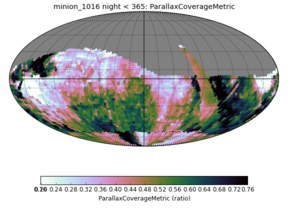
\includegraphics[width=2.0in]{./figs/milkyway/astromPanels/MW_Astrom_paCovge_Baseline_01y_map.png}
  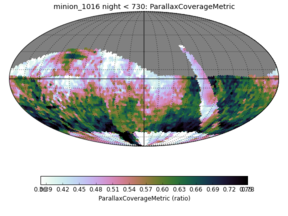
\includegraphics[width=2.0in]{./figs/milkyway/astromPanels/MW_Astrom_paCovge_Baseline_02y_map.png}
  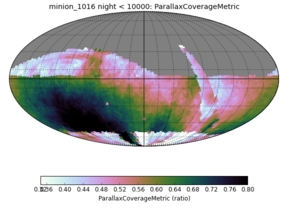
\includegraphics[width=2.0in]{./figs/milkyway/astromPanels/MW_Astrom_paCovge_Baseline_10y_map.png}
  \end{center}
  \begin{center}
  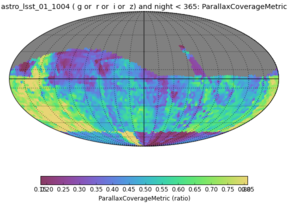
\includegraphics[width=2.0in]{./figs/milkyway/astromPanels/MW_Astrom_paCovge_wfdPlane_01y_map.png}
  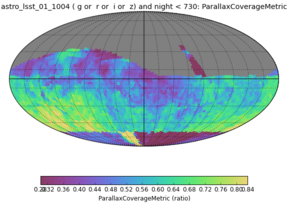
\includegraphics[width=2.0in]{./figs/milkyway/astromPanels/MW_Astrom_paCovge_wfdPlane_02y_map.png}
  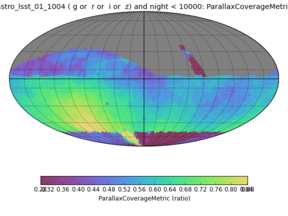
\includegraphics[width=2.0in]{./figs/milkyway/astromPanels/MW_Astrom_paCovge_wfdPlane_10y_map.png}
  \end{center}

  \begin{center}
  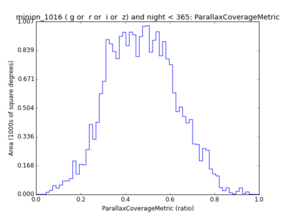
\includegraphics[width=2.0in]{./figs/milkyway/astromPanels/MW_Astrom_paCovge_Baseline_01y_hst.png}
  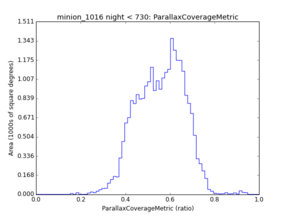
\includegraphics[width=2.0in]{./figs/milkyway/astromPanels/MW_Astrom_paCovge_Baseline_02y_hst.png}
  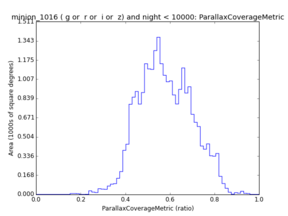
\includegraphics[width=2.0in]{./figs/milkyway/astromPanels/MW_Astrom_paCovge_Baseline_10y_hst.png}
  \end{center}
  \begin{center}
  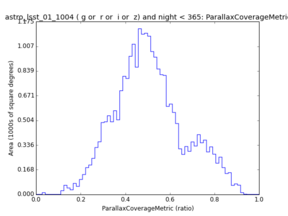
\includegraphics[width=2.0in]{./figs/milkyway/astromPanels/MW_Astrom_paCovge_wfdPlane_01y_hst.png}
  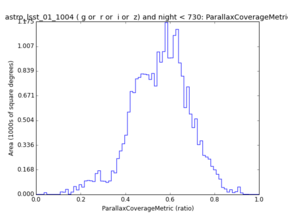
\includegraphics[width=2.0in]{./figs/milkyway/astromPanels/MW_Astrom_paCovge_wfdPlane_02y_hst.png}
  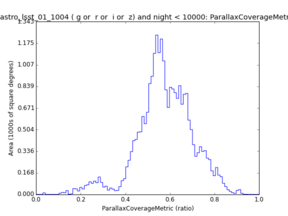
\includegraphics[width=2.0in]{./figs/milkyway/astromPanels/MW_Astrom_paCovge_wfdPlane_10y_hst.png}
  \end{center}
  \caption{Parallax coverage achieved at different epochs within the survey. {\it Top and Third row:} OpSim run \opsimdbref{db:baseCadence}. {\it Second and bottom row:} OpSim run \opsimdbref{db:NormalGalacticPlane} (wide-fast-deep extended to much of the inner Plane). Reading left-right, columns represent: {\it Left column:} all observations within the first 365 days of operation; {\it Middle column:} first two years; {\it right column:} the full 10-year survey. Spatial maps are clipped at 95\%, with histogram horizontal limits (0.0 - 1.0).}
  \label{fig_astrom_ByTime_PACoverage}
\end{figure}

\begin{figure}[ht]
  \begin{center}
  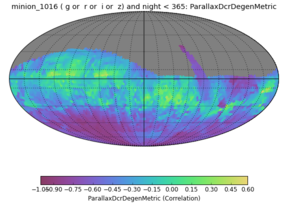
\includegraphics[width=2.0in]{./figs/milkyway/astromPanels/MW_Astrom_paDcrDegen_Baseline_01y_map.png}
  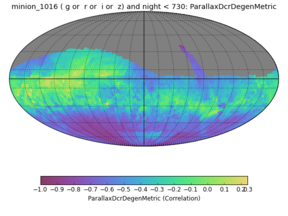
\includegraphics[width=2.0in]{./figs/milkyway/astromPanels/MW_Astrom_paDcrDegen_Baseline_02y_map.png}
  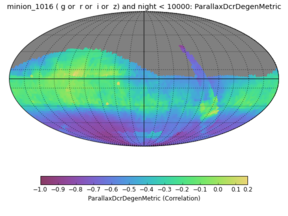
\includegraphics[width=2.0in]{./figs/milkyway/astromPanels/MW_Astrom_paDcrDegen_Baseline_10y_map.png}
  \end{center}
  \begin{center}
  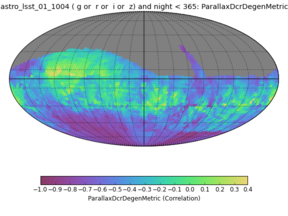
\includegraphics[width=2.0in]{./figs/milkyway/astromPanels/MW_Astrom_paDcrDegen_wfdPlane_01y_map.png}
  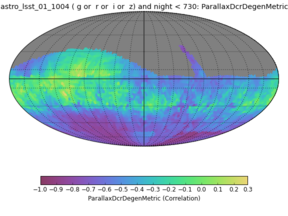
\includegraphics[width=2.0in]{./figs/milkyway/astromPanels/MW_Astrom_paDcrDegen_wfdPlane_02y_map.png}
  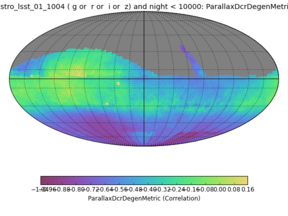
\includegraphics[width=2.0in]{./figs/milkyway/astromPanels/MW_Astrom_paDcrDegen_wfdPlane_10y_map.png}
  \end{center}

  \begin{center}
  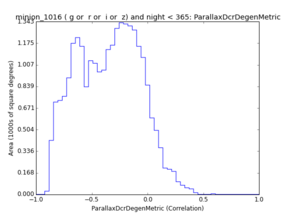
\includegraphics[width=2.0in]{./figs/milkyway/astromPanels/MW_Astrom_paDcrDegen_Baseline_01y_hst.png}
  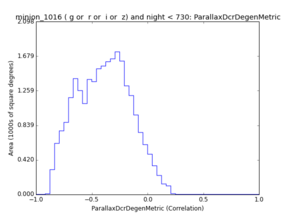
\includegraphics[width=2.0in]{./figs/milkyway/astromPanels/MW_Astrom_paDcrDegen_Baseline_02y_hst.png}
  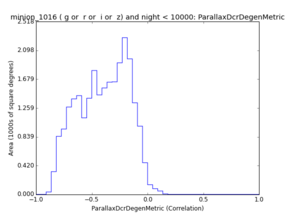
\includegraphics[width=2.0in]{./figs/milkyway/astromPanels/MW_Astrom_paDcrDegen_Baseline_10y_hst.png}
  \end{center}
  \begin{center}
  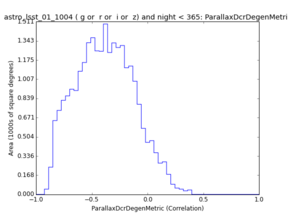
\includegraphics[width=2.0in]{./figs/milkyway/astromPanels/MW_Astrom_paDcrDegen_wfdPlane_01y_hst.png}
  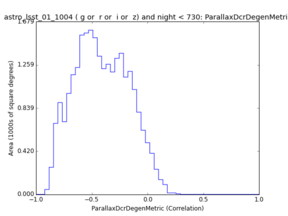
\includegraphics[width=2.0in]{./figs/milkyway/astromPanels/MW_Astrom_paDcrDegen_wfdPlane_02y_hst.png}
  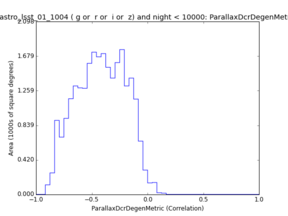
\includegraphics[width=2.0in]{./figs/milkyway/astromPanels/MW_Astrom_paDcrDegen_wfdPlane_10y_hst.png}
  \end{center}
  \caption{Correlation coefficient $\rho$~between parallax and Differential Chromatic Refraction (DCR) up to different epochs within the survey. {\it Top and Third row:} OpSim run \opsimdbref{db:baseCadence}. {\it Second and bottom row:} OpSim run \opsimdbref{db:NormalGalacticPlane} (wide-fast-deep extended to much of the inner Plane). Reading left-right, columns represent: {\it Left column:} all observations within the first 365 days of operation; {\it Middle column:} first two years; {\it right column:} the full 10-year survey. Spatial maps are clipped at 95\%, with histogram horizontal scale set to the range $-1.0 \le \rho \le +1.0$.}
  \label{fig_astrom_ByTime_PADegen}
\end{figure}



\begin{figure}[ht]
  \begin{center}
  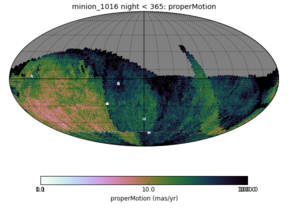
\includegraphics[width=2.0in]{./figs/milkyway/astromPanels/MW_Astrom_pmError_Baseline_01y_map.png}
  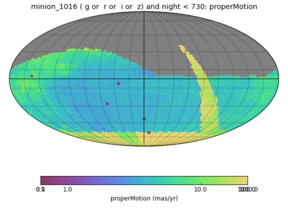
\includegraphics[width=2.0in]{./figs/milkyway/astromPanels/MW_Astrom_pmError_Baseline_02y_map.png}
  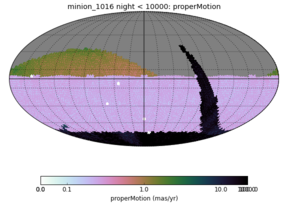
\includegraphics[width=2.0in]{./figs/milkyway/astromPanels/MW_Astrom_pmError_Baseline_10y_map.png}
  \end{center}
  \begin{center}
  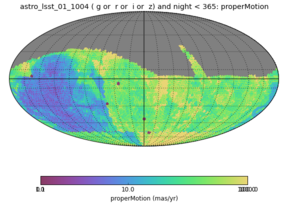
\includegraphics[width=2.0in]{./figs/milkyway/astromPanels/MW_Astrom_pmError_wfdPlane_01y_map.png}
  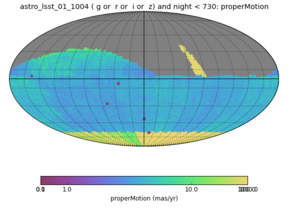
\includegraphics[width=2.0in]{./figs/milkyway/astromPanels/MW_Astrom_pmError_wfdPlane_02y_map.png}
  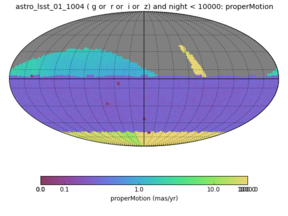
\includegraphics[width=2.0in]{./figs/milkyway/astromPanels/MW_Astrom_pmError_wfdPlane_10y_map.png}
  \end{center}

  \begin{center}
  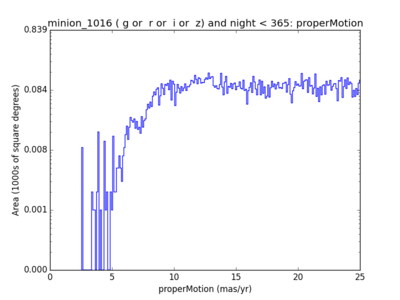
\includegraphics[width=2.0in]{./figs/milkyway/astromPanels/MW_Astrom_pmError_Baseline_01y_hst.png}
  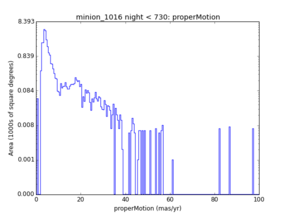
\includegraphics[width=2.0in]{./figs/milkyway/astromPanels/MW_Astrom_pmError_Baseline_02y_hst.png}
  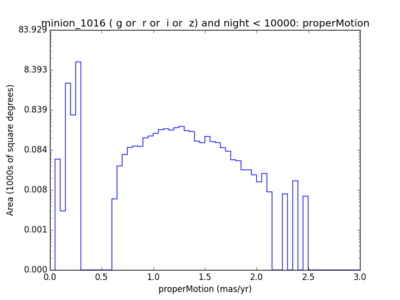
\includegraphics[width=2.0in]{./figs/milkyway/astromPanels/MW_Astrom_pmError_Baseline_10y_hst.png}
  \end{center}
  \begin{center}
  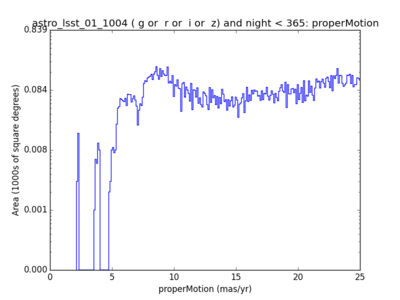
\includegraphics[width=2.0in]{./figs/milkyway/astromPanels/MW_Astrom_pmError_wfdPlane_01y_hst.png}
  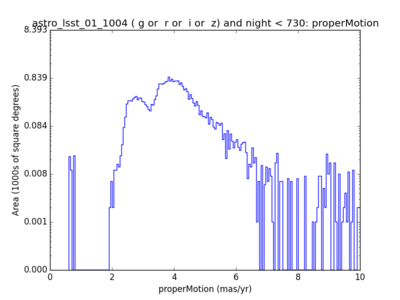
\includegraphics[width=2.0in]{./figs/milkyway/astromPanels/MW_Astrom_pmError_wfdPlane_02y_hst.png}
  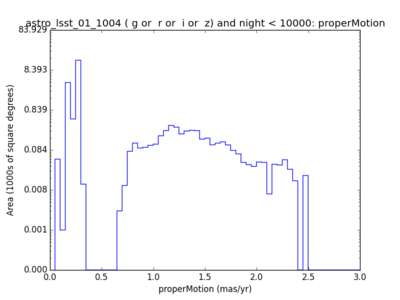
\includegraphics[width=2.0in]{./figs/milkyway/astromPanels/MW_Astrom_pmError_wfdPlane_10y_hst.png}
  \end{center}
  \caption{Proper motion error for a star at $r=21.0$, for different epochs within the survey. Crowding errors are ignored. {\it Top and Third row:} OpSim run \opsimdbref{db:baseCadence}.  {\it Second and bottom row:} OpSim run \opsimdbref{db:NormalGalacticPlane} (wide-fast-deep extended to much of the inner Plane). Reading left-right, columns represent: {\it Left column:} all observations within the first 365 days of operation; {\it Middle column:} first two years; {\it right column:} the full 10-year survey. Spatial maps are clipped at 95\% and a log-scale is used for the maps and histograms. Reading left-right, the horizontal upper limits on the histograms are (25, 10, 3.0) mas yr$^{-1}$, respectively. Note that the histograms do not include the full range of values reported in the maps.}
  \label{fig_astrom_ByTime_pmError}
\end{figure}


\begin{figure}[ht]
  \begin{center}
  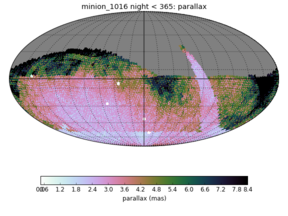
\includegraphics[width=2.0in]{./figs/milkyway/astromPanels/MW_Astrom_paError_Baseline_01y_map.png}
  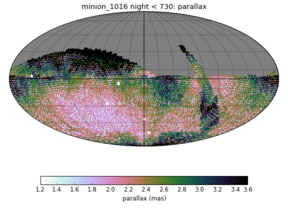
\includegraphics[width=2.0in]{./figs/milkyway/astromPanels/MW_Astrom_paError_Baseline_02y_map.png}
  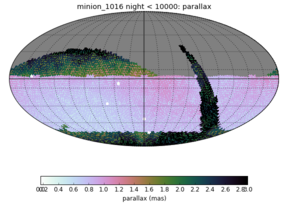
\includegraphics[width=2.0in]{./figs/milkyway/astromPanels/MW_Astrom_paError_Baseline_10y_map.png}
  \end{center}
  \begin{center}
  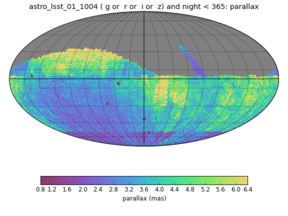
\includegraphics[width=2.0in]{./figs/milkyway/astromPanels/MW_Astrom_paError_wfdPlane_01y_map.png}
  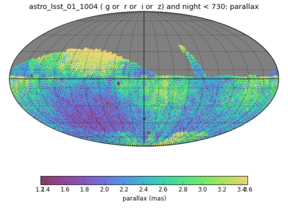
\includegraphics[width=2.0in]{./figs/milkyway/astromPanels/MW_Astrom_paError_wfdPlane_02y_map.png}
  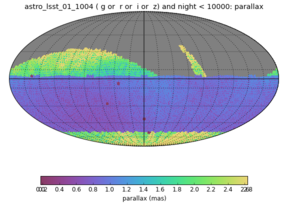
\includegraphics[width=2.0in]{./figs/milkyway/astromPanels/MW_Astrom_paError_wfdPlane_10y_map.png}
  \end{center}

  \begin{center}
  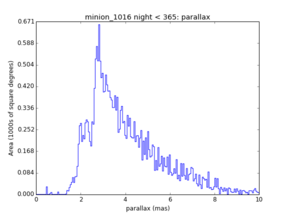
\includegraphics[width=2.0in]{./figs/milkyway/astromPanels/MW_Astrom_paError_Baseline_01y_hst.png}
  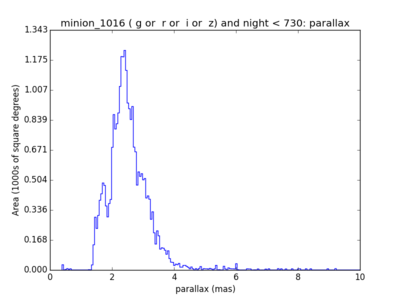
\includegraphics[width=2.0in]{./figs/milkyway/astromPanels/MW_Astrom_paError_Baseline_02y_hst.png}
  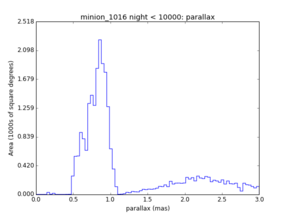
\includegraphics[width=2.0in]{./figs/milkyway/astromPanels/MW_Astrom_paError_Baseline_10y_hst.png}
  \end{center}
  \begin{center}
  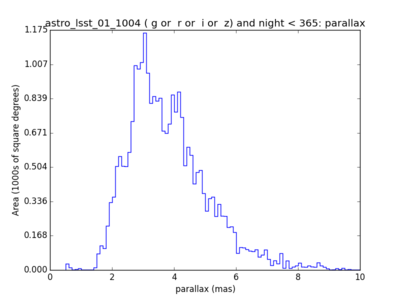
\includegraphics[width=2.0in]{./figs/milkyway/astromPanels/MW_Astrom_paError_wfdPlane_01y_hst.png}
  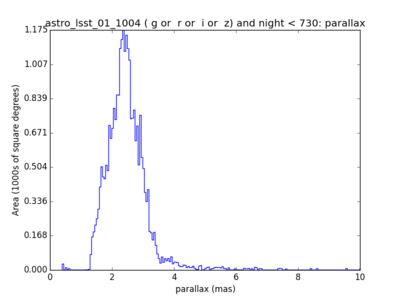
\includegraphics[width=2.0in]{./figs/milkyway/astromPanels/MW_Astrom_paError_wfdPlane_02y_hst.png}
  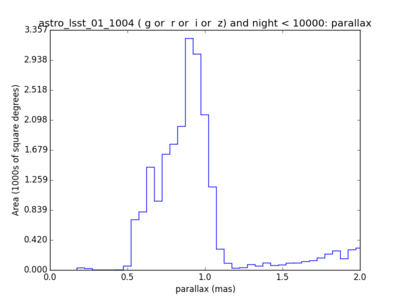
\includegraphics[width=2.0in]{./figs/milkyway/astromPanels/MW_Astrom_paError_wfdPlane_10y_hst.png}
  \end{center}
  \caption{Parallax error for a star at $r=21.0$, for different epochs within the survey. Crowding errors are ignored. {\it Top and Third row:} OpSim run \opsimdbref{db:baseCadence}. {\it Second and bottom row:} OpSim run \opsimdbref{db:NormalGalacticPlane} (wide-fast-deep extended to much of the inner Plane). Reading left-right, columns represent: {\it Left column:} all observations within the first 365 days of operation; {\it Middle column:} first two years; {\it right column:} the full 10-year survey. Spatial maps are clipped at 95\%.  Reading left-right, the horizontal upper limits on the histograms are (10, 10, 2.0) mas, respectively.}
  \label{fig_astrom_ByTime_paError}
\end{figure}

%%% Now for the metrics by filter.
\begin{figure}[ht]
  \begin{center}
  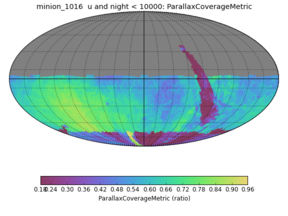
\includegraphics[width=2.0in]{./figs/milkyway/astromPanels/MW_Astrom_paCovge_Baseline_u_map.png}
  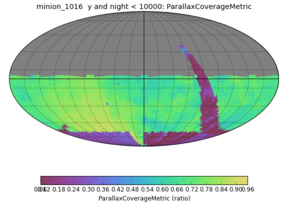
\includegraphics[width=2.0in]{./figs/milkyway/astromPanels/MW_Astrom_paCovge_Baseline_y_map.png}
  \includegraphics[width=2.0in]{./figs/milkyway/astromPanels/MW_Astrom_paCovge_Baseline_10y_map.png}
  \end{center}
  \begin{center}
  \includegraphics[width=2.0in]{./figs/milkyway/astromPanels/MW_Astrom_paCovge_wfdPlane_u_map.png}
  \includegraphics[width=2.0in]{./figs/milkyway/astromPanels/MW_Astrom_paCovge_wfdPlane_y_map.png}
  \includegraphics[width=2.0in]{./figs/milkyway/astromPanels/MW_Astrom_paCovge_wfdPlane_10y_map.png}
  \end{center}

  \begin{center}
  \includegraphics[width=2.0in]{./figs/milkyway/astromPanels/MW_Astrom_paCovge_Baseline_u_hst.png}
  \includegraphics[width=2.0in]{./figs/milkyway/astromPanels/MW_Astrom_paCovge_Baseline_y_hst.png}
  \includegraphics[width=2.0in]{./figs/milkyway/astromPanels/MW_Astrom_paCovge_Baseline_10y_hst.png}
  \end{center}
  \begin{center}
  \includegraphics[width=2.0in]{./figs/milkyway/astromPanels/MW_Astrom_paCovge_wfdPlane_u_hst.png}
  \includegraphics[width=2.0in]{./figs/milkyway/astromPanels/MW_Astrom_paCovge_wfdPlane_y_hst.png}
  \includegraphics[width=2.0in]{./figs/milkyway/astromPanels/MW_Astrom_paCovge_wfdPlane_10y_hst.png}
  \end{center}
  \caption{Parallax coverage achieved for three extremes of object color, over the full 10-year survey. {\it Top and Third row:} OpSim run \opsimdbref{db:baseCadence}. {\it Second and bottom row:} OpSim run \opsimdbref{db:NormalGalacticPlane} (wide-fast-deep extended to much of the inner Plane). Reading left-right, columns represent: {\it Left column:} Objects detected only in the bluest filter; {\it Middle column:} objects detected only in the reddest filter; {\it Right column:} objects detected in all filters. Spatial maps are clipped at 95\%, with histogram horizontal limits (0.0 - 1.0).}
  \label{fig_astrom_ByFilter_PACoverage}
\end{figure}

\begin{figure}[ht]
  \begin{center}
  \includegraphics[width=2.0in]{./figs/milkyway/astromPanels/MW_Astrom_paDcrDegen_Baseline_u_map.png}
  \includegraphics[width=2.0in]{./figs/milkyway/astromPanels/MW_Astrom_paDcrDegen_Baseline_y_map.png}
  \includegraphics[width=2.0in]{./figs/milkyway/astromPanels/MW_Astrom_paDcrDegen_Baseline_10y_map.png}
  \end{center}
  \begin{center}
  \includegraphics[width=2.0in]{./figs/milkyway/astromPanels/MW_Astrom_paDcrDegen_wfdPlane_u_map.png}
  \includegraphics[width=2.0in]{./figs/milkyway/astromPanels/MW_Astrom_paDcrDegen_wfdPlane_y_map.png}
  \includegraphics[width=2.0in]{./figs/milkyway/astromPanels/MW_Astrom_paDcrDegen_wfdPlane_10y_map.png}
  \end{center}

  \begin{center}
  \includegraphics[width=2.0in]{./figs/milkyway/astromPanels/MW_Astrom_paDcrDegen_Baseline_u_hst.png}
  \includegraphics[width=2.0in]{./figs/milkyway/astromPanels/MW_Astrom_paDcrDegen_Baseline_y_hst.png}
  \includegraphics[width=2.0in]{./figs/milkyway/astromPanels/MW_Astrom_paDcrDegen_Baseline_10y_hst.png}
  \end{center}
  \begin{center}
  \includegraphics[width=2.0in]{./figs/milkyway/astromPanels/MW_Astrom_paDcrDegen_wfdPlane_u_hst.png}
  \includegraphics[width=2.0in]{./figs/milkyway/astromPanels/MW_Astrom_paDcrDegen_wfdPlane_y_hst.png}
  \includegraphics[width=2.0in]{./figs/milkyway/astromPanels/MW_Astrom_paDcrDegen_wfdPlane_10y_hst.png}
  \end{center}
  \caption{Correlation coefficient $\rho$~between parallax and Differential Chromatic Refraction (DCR), selecting filters for three extremes of object color, over the full 10-year survey. {\it Top and Third row:} OpSim run \opsimdbref{db:baseCadence}. {\it Second and bottom row:} OpSim run \opsimdbref{db:NormalGalacticPlane} (wide-fast-deep extended to much of the inner Plane). Reading left-right, columns represent: {\it Left column:} Objects detected only in the bluest filter; {\it Middle column:} objects detected only in the reddest filter; {\it Right column:} objects detected in all filters. Spatial maps are clipped at 95\%, with histogram horizontal scale set to the range $-1.0 \le \rho \le +1.0$.}
  \label{fig_astrom_ByFilter_PADegen}
\end{figure}

\begin{figure}[ht]
  \begin{center}
  \includegraphics[width=2.0in]{./figs/milkyway/astromPanels/MW_Astrom_pmError_Baseline_u_map.png}
  \includegraphics[width=2.0in]{./figs/milkyway/astromPanels/MW_Astrom_pmError_Baseline_y_map.png}
  \includegraphics[width=2.0in]{./figs/milkyway/astromPanels/MW_Astrom_pmError_Baseline_10y_map.png}
  \end{center}
  \begin{center}
  \includegraphics[width=2.0in]{./figs/milkyway/astromPanels/MW_Astrom_pmError_wfdPlane_u_map.png}
  \includegraphics[width=2.0in]{./figs/milkyway/astromPanels/MW_Astrom_pmError_wfdPlane_y_map.png}
  \includegraphics[width=2.0in]{./figs/milkyway/astromPanels/MW_Astrom_pmError_wfdPlane_10y_map.png}
  \end{center}

  \begin{center}
  \includegraphics[width=2.0in]{./figs/milkyway/astromPanels/MW_Astrom_pmError_Baseline_u_hst.png}
  \includegraphics[width=2.0in]{./figs/milkyway/astromPanels/MW_Astrom_pmError_Baseline_y_hst.png}
  \includegraphics[width=2.0in]{./figs/milkyway/astromPanels/MW_Astrom_pmError_Baseline_10y_hst.png}
  \end{center}
  \begin{center}
  \includegraphics[width=2.0in]{./figs/milkyway/astromPanels/MW_Astrom_pmError_wfdPlane_u_hst.png}
  \includegraphics[width=2.0in]{./figs/milkyway/astromPanels/MW_Astrom_pmError_wfdPlane_y_hst.png}
  \includegraphics[width=2.0in]{./figs/milkyway/astromPanels/MW_Astrom_pmError_wfdPlane_10y_hst.png}
  \end{center}
  \caption{Proper motion error for a star at apparent magnitude $m=21.0$, for three extremes of object color and assessed over the full survey. Crowding errors are ignored. {\it Top and Third row:} OpSim run \opsimdbref{db:baseCadence}. {\it Second and bottom row:} OpSim run \opsimdbref{db:NormalGalacticPlane} (wide-fast-deep extended to much of the inner Plane). Reading left-right, columns represent: {\it Left column:} Objects detected only in the bluest filter; the fiducial object has apparent magnitude $u=21.0$; {\it Middle column:} objects detected only in the reddest filter (so $y = 21.0$); {\it Right column:} objects detected in all filters (using $r=21.0$~and a ``flat'' spectrum within sims\_maf). Spatial maps are clipped at 95\% and a log-scale is used for both the spatial maps and histograms. Reading left-right, the horizontal upper limits on the histograms are (4.0, 4.0, 3.0) mas yr$^{-1}$, respectively. Note that the histograms do not include the full range of values reported in the maps.}
  \label{fig_astrom_ByFilter_pmError}
\end{figure}

\begin{figure}[ht]
  \begin{center}
  \includegraphics[width=2.0in]{./figs/milkyway/astromPanels/MW_Astrom_paError_Baseline_u_map.png}
  \includegraphics[width=2.0in]{./figs/milkyway/astromPanels/MW_Astrom_paError_Baseline_y_map.png}
  \includegraphics[width=2.0in]{./figs/milkyway/astromPanels/MW_Astrom_paError_Baseline_10y_map.png}
  \end{center}
  \begin{center}
  \includegraphics[width=2.0in]{./figs/milkyway/astromPanels/MW_Astrom_paError_wfdPlane_u_map.png}
  \includegraphics[width=2.0in]{./figs/milkyway/astromPanels/MW_Astrom_paError_wfdPlane_y_map.png}
  \includegraphics[width=2.0in]{./figs/milkyway/astromPanels/MW_Astrom_paError_wfdPlane_10y_map.png}
  \end{center}

  \begin{center}
  \includegraphics[width=2.0in]{./figs/milkyway/astromPanels/MW_Astrom_paError_Baseline_u_hst.png}
  \includegraphics[width=2.0in]{./figs/milkyway/astromPanels/MW_Astrom_paError_Baseline_y_hst.png}
  \includegraphics[width=2.0in]{./figs/milkyway/astromPanels/MW_Astrom_paError_Baseline_10y_hst.png}
  \end{center}
  \begin{center}
  \includegraphics[width=2.0in]{./figs/milkyway/astromPanels/MW_Astrom_paError_wfdPlane_u_hst.png}
  \includegraphics[width=2.0in]{./figs/milkyway/astromPanels/MW_Astrom_paError_wfdPlane_y_hst.png}
  \includegraphics[width=2.0in]{./figs/milkyway/astromPanels/MW_Astrom_paError_wfdPlane_10y_hst.png}
  \end{center}
  \caption{Parallax error for a star at apparent magnitude $m=21.0$, for three extremes of object color and assessed over the full survey. Crowding errors are ignored. {\it Top and Third row:} OpSim run \opsimdbref{db:baseCadence}. {\it Second and bottom row:} OpSim run \opsimdbref{db:NormalGalacticPlane} (wide-fast-deep extended to much of the inner Plane). Reading left-right, columns represent: {\it Left column:} Objects detected only in the bluest filter; the fiducial object has apparent magnitude $u=21.0$; {\it Middle column:} objects detected only in the reddest filter (so $y = 21.0$); {\it Right column:} objects detected in all filters (using $r=21.0$~and a ``flat'' spectrum within sims\_maf). Spatial maps are clipped at 95\%. Reading left-right, the horizontal upper limits on the histograms are (10, 10, 2.0) mas, respectively. Note that the histograms do not include the full range of values reported in the maps.}
  \label{fig_astrom_ByFilter_paError}
\end{figure}

\subsubsection{Figures of Merit depending on the Metrics}

Building on the first-order metrics above, this subsection communicates scientific figures of merit for the cases identified in \autoref{sec:\secname:MW_Astrometry_measurements} above.

Table \ref{tab_SummaryMWAstrometry} summarizes the Figures of Merit
(FoMs) for Astrometry science cases. At the time of writing, FoMs have
been implemented to summarize the random uncertainty in proper motion
and parallax, for two regions experiencing extreme values of these
quantities: the inner Plane (conservatively defined in this section as
$|b| \lesssim 7^o$~and $|l| \lesssim 80^o$), and the main survey
(excluding the inner plane and the Southern Polar region, taken
here as $\delta_{2000.0} < -60.0^o$). Figure
\ref{fig_astrom_RegionSelKey} illustrates these selection-regions on
the sky. These form FoM 1.1-1.4, and have to-date been run for the
OpSim runs \opsimdbref{db:baseCadence} (Baseline cadence),
\opsimdbref{db:opstwoPS} (similar to PanSTARRS-1), and the
recently-completed \opsimdbref{db:NormalGalacticPlane} (which applies
Wide-Fast-Deep cadence to much of the inner Galactic Plane). From the point of
view of parallax and proper motion, the latter two strategies do not
negatively impact the non-plane regions, but they {\it substantially}
improve the sampling for proper motions and parallax (again,
neglecting the effects of spatial crowding).

FoM 1.5 in Table \ref{tab_SummaryMWAstrometry} reports the total number of fields with Parallax/Hour-angle correlation $|\rho| < 0.7$.

At the time of writing, FoMs 2-5 in Table
\ref{tab_SummaryMWAstrometry} are still at the specification stage,
and are described in Section
\ref{sec:\secname:MW_Astrometry_furtherwork}.

%%%% Figures used as ``key'' for the astrometry FoMs:

\begin{figure}[h]
  \begin{center}
    \includegraphics[width=2.0in]{./figs/milkyway/astromPanels/MW_Astrom_FoM_properMotion_minion_1016_all_skymap.png}
  \includegraphics[width=2.0in]{./figs/milkyway/astromPanels/MW_Astrom_FoM_properMotion_minion_1016_plane_skymap.png}
  \includegraphics[width=2.0in]{./figs/milkyway/astromPanels/MW_Astrom_FoM_properMotion_minion_1016_nonPlane_skymap.png}
    \end{center}
  \caption{Selection regions for the Astrometry Figures of Merit (FoMs) 1.1-1.4. Figures of Merit 1.1 and 1.3 refer to the ``main survey'' region shown in the middle panel (which for the FoM also avoids the region of the South Galactic Pole). The right panel shows the inner Plane region to which FoMs 1.2 \& 1.4 refer. The left-hand panel shows the entire survey region for reference. This example shows run \opsimdbref{db:baseCadence}. See Table \ref{tab_SummaryMWAstrometry} and Section \ref{sec:\secname:MW_Astrometry_metrics}.}
  \label{fig_astrom_RegionSelKey}
\end{figure}

\subsection{Topics that will need to be addressed}
\label{sec:\secname:MW_Astrometry_furtherwork}

Here we present suggestions for further work, first on figures of
merit for the science cases, and then on additional Metrics for LSST's
astrometric performance.

\subsubsection{Further work on science Figures of Merit}
%\medskip

At the time of writing, the Figures of Merit for both the highlighted
Science cases need to be implemented and applied to OpSim output,
preferably in a format that can be summarized in a single Table in
this section. These figures of merit are discussed above in Section
\ref{sec:\secname:MW_Astrometry_metrics} (particularly for the Halo
Streams science project). Figures of merit for the two science cases
might be:
\begin{itemize}
  \item[1.] Number of streams that LSST can discover via their proper motions;
\item[2.] Uncertainty and bias in the thin and thick disk differential age measurement when using white dwarfs from each population as tracers.
\end{itemize}

Given the diversity of science cases that use local Solar Neighborhood
populations as tracers, it may be advantageous to subdivide the Solar
Neighborhood projects into further figures of merit. Two further example
figures of merit might then be:
\begin{itemize}
  \item[3.] Uncertainty and bias in the Brown Dwarf mass function using Solar Neighborhood tracers;
   \item[4.] Uncertainty and bias in the thickness in the main sequence of M-dwarfs within 25pc from the Sun, once variability has been characterized and removed.
\end{itemize}

%%%% SUMMARY TABLE FOR THIS SECTION

\begin{table}
  \begin{tabular}{l|p{4.8cm}|p{1.1cm}|p{1.1cm}|p{1.1cm}|c|p{3.5cm}}
    FoM & Brief description & {\rotatebox{90}{\opsimdbref{db:baseCadence} }} & {\rotatebox{90}{\opsimdbref{db:opstwoPS} }} & {\rotatebox{90}{\opsimdbref{db:NormalGalacticPlane}   }} &  {\rotatebox{90}{future run 2}} & Notes \\
    \hline
    1.1 & \footnotesize{Median parallax error at $r=21$ (main survey)}      & 0.69  & 0.72 & 0.69 & - &
%\footnotesize{Summarize the presentation in Figures \ref{fig_astrom_ByTime_PACoverage}-\ref{fig_astrom_ByFilter_paError} }
\footnotesize{See region definitions in Figure \ref{fig_astrom_RegionSelKey}.}
\\
    1.2. & \footnotesize{Median parallax error at $r=21$ (plane)}   & 2.68 & {\bf 0.91} & {\bf 0.89} & - &
\footnotesize{Smaller values are better.}\\
    1.3. & \footnotesize{Median proper motion error at $r=21$ (main survey)}  & 0.19 & 0.19 & 0.19 & - &
%\footnotesize{Take median of Figure \ref{fig_astrom_ByTime_pmError} over the ``plane'' region.}
\\
    1.4. & \footnotesize{Median proper motion error at $r=21$ (plane)} & 16.7
%$^\dagger$
& {\bf 0.26} & {\bf 0.25} & - &
%\footnotesize{$^\dagger$no, this is not a typo.}
\\
1.5. & \footnotesize{Fields with Parallax-DCR correlation coefficient $\rho \ge 0.7$~/ total fields} & \footnotesize{ \bf{3486} / \bf {31116} } & \footnotesize{3586 / 30107} & \footnotesize{3690 / 31116} & - & \footnotesize{Smaller is better. Value reported after full 10 years of survey for $griz$~detections.}  \\
    \hline
    2.1. & \footnotesize{Number of streams LSST can discover via proper motions} & - & - & - & - &  - \\
    3.1. & \footnotesize{Uncertainty and bias in thin- and thick-disk differential age measurement via white dwarfs} & - & - & - & - &  - \\
    4.1. & \footnotesize{Uncertainty and bias in brown dwarf mass function from the Solar Neighborhood}  & - & - & - & - & \footnotesize{Using astrometry metrics for objects detected only in the reddest filter(s)} \\
    4.2. & \footnotesize{Uncertainty and bias in white dwarf mass function from the Solar Neighborhood}  & - & - & - & - & \footnotesize{Using astrometry metrics for objects detected only in the bluest filter(s)} \\
    5.1. & \footnotesize{Uncertainty and bias in Solar Neighborhood M-dwarf thickness on the MS}  & - & - & - & - &  - \\
\end{tabular}
\caption{Summary of Figures of Merit for the Milky Way Astrometry science cases. The best value of each FoM is indicated in bold. Runs \opsimdbref{db:baseCadence} and \opsimdbref{db:opstwoPS} refer to the Baseline and PanSTARRS-like strategies, respectively. Column \opsimdbref{db:NormalGalacticPlane} refers to a recently-completed OpSim run that includes the Plane in Wide-Fast-Deep observations. See \autoref{sec:MW_Astrometry}.}
\label{tab_SummaryMWAstrometry}
\end{table}


%%%% SUMMARY TABLE FINISHES HERE


\subsubsection{Further work on Astrometry Metrics}

The MAF metrics presented in Sections \ref{sec:\secname:MW_Astrometry_OpSim} and \ref{sec:\secname:MW_Astrometry_metrics} are only part of the
study of LSST's predicted astrometric performance.  Detailed simulations
and studies need to be done in many other areas as part of the
prediction and verification of LSST's astrometric performance.  Among
the most important are the following.
\begin{itemize}
\item How well do galaxies perform as astrometric reference objects? Are certain shapes or colors better than others? What is the
surface density of ``good" astrometric reference galaxies as a function of filter?
\item How well can we identify optically point-like QSOs that will be useful in matching the optical reference frame to the ICRS?
%\item Given the LSST exposure time, site, and physical characteristics, how can we mitigate the limitations on astrometric accuracy imposed by the seeing and local atmospheric turbulence?
\item How does the astrometric performance depend on stellar density? If there are fields in which photometry is only possible via difference imaging, what are the limitations
on astrometry in these fields?
%\item What tools do we need to compare the general and specific agreement between the {\it Gaia} results and the LSST results?
\item Does the ``brighter-wider" effect in the deep-depletion CCDs introduce a magnitude term into the centroid positions?
\end{itemize}

% ====================================================================

\subsection{Conclusions}

Here we answer the ten questions posed in
\autoref{sec:intro:evaluation:caseConclusions}:

\begin{description}

\item[Q1:] {\it Does the science case place any constraints on the
tradeoff between the sky coverage and coadded depth? For example, should
the sky coverage be maximized (to $\sim$30,000 deg$^2$, as e.g., in
Pan-STARRS) or the number of detected galaxies (the current baseline but
with 18,000 deg$^2$)?}

\new{ \item[A1:] We do expect tradeoffs between depth and sky
  coverage, but we do not yet have the FoM evaluations to set
  quantitative constraints. For example, we expect some combination of
  depth and survey volume would optimize the completeness to objects
  among the populations in the Solar Neighborhood. More generally,
  perhaps, in fields away from the galactic mid-plane, the
  lengthscales over which the proper motion zeropoints can be
  accurately constrained will depend on the spatial density of
  well-measured background galaxies (finer lengthscale corresponding
  to greater co-added depth). The depth must therefore be sufficient
  to sample enough of these galaxies to constrain variations of
  astrometric zeropoint on lengthscales at least as fine as those
  imposed by the LSST system itself (or the atmosphere, whichever is
  finer). We anticipate that this tradeoff can be informed by
  simulation under a set of assumptions for these variations.}

\item[Q2:] {\it Does the science case place any constraints on the
tradeoff between uniformity of sampling and frequency of  sampling? For
example, a rolling cadence can provide enhanced sample rates over a part
of the survey or the entire survey for a designated time at the cost of
reduced sample rate the rest of the time (while maintaining the nominal
total visit counts).}

\new{ \item[A2:] Yes, although for astrometry the language of these
  constraints is slightly different. The parallactic ellipse must be
  sufficiently covered, the correlation between hour angle and
  parallax factor must be minimized, and the visits must be
  sufficiently distributed (both within a year and over the ten-year
  time baseline) to produce the best precision in both proper motion and parallax. See Section \ref{sec:MW_Astrometry:MW_Astrometry_metrics}}.

\item[Q3:] {\it Does the science case place any constraints on the
tradeoff between the single-visit depth and the number of visits
(especially in the $u$-band where longer exposures would minimize the
impact of the readout noise)?}

\new{ \item[A3:] More visits at the standard exposure time are
  generally preferred to a few visits with longer exposures, in order
  to achieve as broad a temporal coverage as possible (see Section
  \ref{sec:MW_Astrometry:MW_Astrometry_metrics}). The $u$-band itself
  is likely to be of limited use for astrometry (except possibly for
  extremely blue objects with little signal in any of the other
  filters) due to differential chromatic refraction (DCR), however of
  course $u$-band will still be useful for photometric constraints.}

\item[Q4:] {\it Does the science case place any constraints on the
Galactic plane coverage (spatial coverage, temporal sampling, visits per
band)?}

\new{ \item[A4:] Not for the example of detecting Galactic Halo
  streams via proper motions (Section
  \ref{sec:MW_Astrometry:MW_Astrometry_measurements}). For the Solar
  Neighborhood populations, avoiding the inner Galactic mid-plane
  would obviously reduce the completeness of the census of nearby
  objects with parallax determinations due to the reduction in total
  area surveyed. However, this reduction may be incremental rather
  than serious. The impact of an inner-plane zone of avoidance on the
  recovery of the parameters describing these constituent populations
  has not yet been evaluated. Of course, this all changes for
  astrometry of objects of interest that lie in the inner plane (see
  also Section \ref{sec:MW_Disk}), where (for example) the reduced
  proper motion will be a useful diagnostic. At present, however, the
  performance of the LSST software stack towards crowded fields is
  as-yet unknown. As this performance becomes better understood, it
  will be possible to quantitatively compare strategies for astrometry
  towards the inner plane.}

\item[Q5:] {\it Does the science case place any constraints on the
fraction of observing time allocated to each band?}

\new{ \item[A5:] Yes, but indirectly through the requirement to
  measure all the populations of interest in the Solar
  Neighborhood. Making the assumption that this science case requires
  parallax measurements for extremely blue objects as well as
  extremely red objects, which might each be measurable only in a
  single very red or blue filter, would suggest at a minimum that the
  coverage considerations of Section
  \ref{sec:MW_Astrometry:MW_Astrometry_metrics} be applied to
  observations in $u$~and $Y$ filters separately, as well as at least
  one mid-range filter. However the quantitative impact on population
  recovery from various filter-distributions has yet to be assessed at
  this date. Further work is needed to determine if the increased
  sensitivity of $u$-band astrometry to DCR relative to $g$-band would
  prevent its use for astrometry.}

\item[Q6:] {\it Does the science case place any constraints on the
cadence for deep drilling fields?}

\new{ \item[A6:] If precision astrometry is desired for the deep drilling fields, then the considerations of Section \ref{sec:MW_Astrometry:MW_Astrometry_metrics} apply to those fields as well.}

\item[Q7:] {\it Assuming two visits per night, would the science case
benefit if they are obtained in the same band or not?}

\new{ \item[A7:] While detailed investigation is still pending, we
  expect that using different filters within the same night would be
  preferred to allow better constraint of DCR effects. Doing different
  filters on the same night might reduce the number of free parameters
  (like seeing and parallax factor) and give more pairs for direct
  filter-A vs. filter-B astrometry.}

\item[Q8:] {\it Will the case science benefit from a special cadence
prescription during commissioning or early in the survey, such as:
acquiring a full 10-year count of visits for a small area (either in all
the bands or in a  selected set); a greatly enhanced cadence for a small
area?}

\new{ \item[A8:] It is vital for astrometry that at least a few fields
  be observed with both sufficient parallax factor coverage and
  sufficient number of visits, early in the survey, to demonstrate
  parallax precision specified in the Science Requirements
  Document. In these fields, sufficient exposures must be reserved for
  the entire 10-year survey baseline so that proper motion precision
  is not too badly compromised in these fields. This combination of
  factors may require dedicated commissioning observations of these
  fields in addition to the 10-year survey operations. In addition,
  however, at least a few fields must be observed at a variety of
  values of single-visit achieved depth, and FWHM, in order to
  constrain the degree to which FWHM will actually predict the
  achieved astrometric precision (see also the answer to Q10
  below). This second set of requirements may also be best served by
  dedicated commissioning observations.}

\item[Q9:] {\it Does the science case place any constraints on the
sampling of observing conditions (e.g., seeing, dark sky, airmass),
possibly as a function of band, etc.?}

\new{ \item[A9:] The observations need to be planned in such a way
  that the correlation between parallax and hour-angle is minimized,
  to avoid deneracies between the motion due to atmospheric refraction and the motion that is sought due to parallax. See
  Section \ref{sec:MW_Astrometry:MW_Astrometry_metrics}.}

\item[Q10:] {\it Does the case have science drivers that would require
real-time exposure time optimization to obtain nearly constant
single-visit limiting depth?}

\new{ \item[A10:] While optimization on an exposure-to-exposure basis
  is perhaps unlikely, {\it selection} between observations in
  response to conditions (on a timescale of perhaps 10 minutes) will
  be crucial to maximize achieved astrometric precision. The rules by
  which this selection would proceed, still need to be charted. For
  example, while maintaining limiting depth might suggest shorter
  exposure times when the FWHM is narrow, this may not translate to
  improved astrometric error across an LSST chip, because the
  lengthscales of the turbulence driving the FWHM is not the same as
  that of the turbulence driving astrometric error across an LSST chip.}

\end{description}

\navigationbar

% --------------------------------------------------------------------
